%\documentclass{beamer}
%\usepackage{minijs}
%\usepackage{here}
%\mode<presentation>{
%  \usetheme{Antibes}
%  \usecolortheme{beaver}
%  \setbeamercovered{transparent}
%}
\documentclass[13pt,dvipdfmx]{beamer}
\usepackage[english]{babel}
% pdfの栞の字化けを防ぐ
\AtBeginDvi{\special{pdf:tounicode EUC-UCS2}}
% テーマ
\usetheme{metropolis}
\usepackage{caption}
\setbeamertemplate{navigation symbols}{} 
\usepackage{graphicx}
%\usepackage[dvipdfmx]{graphicx}
\usepackage{amsmath}
\usepackage{amssymb}
\usepackage{txfonts}
\usepackage{colortbl}
\usepackage{svg}
\renewcommand{\familydefault}{\sfdefault}
\renewcommand{\kanjifamilydefault}{\gtdefault}
\setbeamerfont{title}{size=\large,series=\bfseries}
\setbeamerfont{frametitle}{size=\large,series=\bfseries}
\setbeamertemplate{frametitle}[default][center]
\usefonttheme{professionalfonts} 


%1ページめ
\title{通信ゼミナール}
\subtitle{クラスタリング手法の評価}
\author{池辺 颯一}
\institute{芝浦工業大学 工学部 通信工学科}
\date{2018年12月12日}

\begin{document}
\begin{frame}\frametitle{}
 \titlepage
\end{frame}

\begin{frame}\frametitle{概要・背景}
\begin{itemize}
 \item 情報化社会の発展によりデータが複雑かつ膨大に
 \item ビッグデータを人の手で分類するのは難しい
 \item それらのデータを自動的に分類するクラスタリングに着目
\end{itemize}
\vspace{5mm}
\begin{figure}[htbp]
 \begin{minipage}{0.4\hsize}
  \begin{center}
   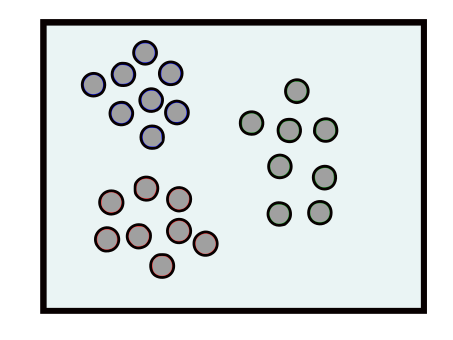
\includegraphics[width=40mm]{before_clustering.png}
  \end{center}
  \captionsetup{labelformat=empty,labelsep=none}
  \caption{クラスタリング前}
  \label{fig:one}
 \end{minipage}
\hspace{1cm}
 \begin{minipage}{0.4\hsize}
  \begin{center}
   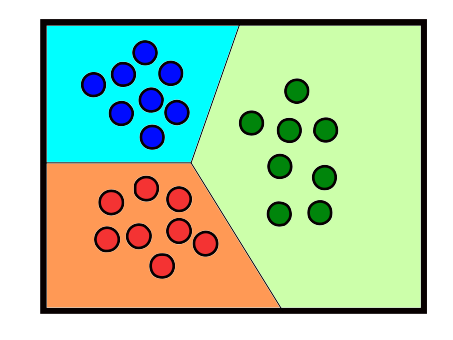
\includegraphics[width=40mm]{after_clustering.png}
  \end{center}
  \captionsetup{labelformat=empty,labelsep=none}
  \caption{クラスタリング後}
  \label{fig:two}
 \end{minipage}
\end{figure}
\end{frame}

\begin{frame}\frametitle{目的・目標}
\begin{block}{目的}
\begin{itemize}
 \item クラスタリング手法の1つであるFussy c-meansにクラスタサイズ調整変数を導入した最適化問題の中から最も精度が高いものを発見する
\end{itemize}
\end{block}
\vspace{4mm}
\begin{block}{目標}
\begin{itemize}
 \item 各クラスタリング手法のプログラムをC++を用いて開発
 \item プログラムの実行結果からクラスタリング精度を評価
\end{itemize}
\end{block}
\end{frame}

\begin{frame}\frametitle{実験対象}
  \begin{block}{既存手法}
   \begin{itemize}
    \item sFCM
    \item pFCM
    \item eFCM
   \end{itemize}
  \end{block}
 \begin{block}{比較対象手法}
   \begin{itemize}
    \item クラスタサイズ調整変数を導入
    \item sFCMA
    \item pFCMA
    \item eFCMA
   \end{itemize}
 \end{block}
\end{frame}

\begin{frame}\frametitle{クラスタリングの最適化問題}
  \begin{block}{eFCMA}
  \quad$\underset{u,v,\alpha}{\text{minimize}}$
    $\sum_{i=1}^C\sum_{k=1}^Nu_{i,k}||x_k-v_i||_2^2+\lambda^{-1}\sum_{i=1}^C\sum_{k=1}^Nu_{i,k}\log\Bigl(\frac{u_{i,k}}{\alpha_{i}}\Bigl)$
  \end{block}
  \begin{center}
\begin{tabular}{c||c|c||c} \hline
	{$N$}&データ数&{$x_k$}&データ数 \\ \hline
	{$C$}&クラスタ数&{$v_i$}&クラスタ中心\\ \hline
	{$\lambda$}&ファジィ化パラメータ&{$u_{i,k}$}&帰属度 \\ \hline
	{$\alpha_i$}&クラスタサイズ調整変数\\ \hline
\end{tabular}
\end{center}
   %% \begin{align*}
   %%   v_{i}=\frac{\sum_{k=1}^Nu_{i,k}x_{k}}{\quad\sum_{k=1}^Nu_{i,k}},\\
   %% u_{i,k}&=\frac{\pi_{i}\exp(-\lambda||x_k-v_i||_2^2)}{\sum_{j=1}^C\pi_{j}\exp(-\lambda||x_k-v_j||_2^2)},\\
   %%  \alpha_{i}&=\frac{\sum_{k=1}^Nu_{i,k}}{\quad N}.\\
   %% \end{align*}
\end{frame}

\begin{frame}\frametitle{クラスタリングの最適化問題}
  \begin{block}{qFCMA}
    \quad$\underset{u,v,\alpha}{\text{minimize}}$
    $\sum_{i=1}^C\sum_{k=1}^N(\alpha_{i})^{1-m}(u_{i,k})^m||x_k-v_i||_2^2$\\
    \qquad\qquad\qquad\qquad$+\frac{\lambda^{-1}}{m-1}\sum_{i=1}^C\sum_{k=1}^N(\alpha_{i})^{1-m}(u_{i,k})^m$
  \end{block}
  \begin{center}
\begin{tabular}{c||c|c||c} \hline
	{$N$}&データ数&{$x_k$}&データ数 \\ \hline
	{$C$}&クラスタ数&{$v_i$}&クラスタ中心\\ \hline
	{$\lambda,m$}&ファジィ化パラメータ&{$u_{i,k}$}&帰属度 \\ \hline
	{$\alpha_i$}&クラスタサイズ調整変数\\ \hline
\end{tabular}
\end{center}
   %% \begin{align*}
   %%  v_{i}=\frac{\sum_{k=1}^N(u_{i,k})^mx_{k}}{\quad\sum_{k=1}^N(u_{i,k})^{m}},\\
   %%  u_{i,k}&=\frac{\alpha_{i}(1+\lambda(1-m)||x_i-v_k||_2^2)^\frac{1}{1-m}}{\quad\sum_{j=1}^C\alpha_{j}(1+\lambda(1-m)||x_j-v_k||_2^2)^\frac{1}{1-m}},\\
   %%  \alpha_{i}&=\frac{1}{\sum_{j=1}^C\left(\sum_{k=1}^N\frac{(u_{j,k})^m(1-\lambda(1-m)d_{j,k})}{(u_i,k)^m(1-\lambda(1-m)d_{i,k})}\right)^{\frac{1}{m}}}.\\
   %% \end{align*}
  \end{frame}

\begin{frame}\frametitle{クラスタリングの最適化問題}
  \begin{block}{sFCMA}
    \quad$\underset{u,v,\alpha}{\text{minimize}}$
    $\sum_{i=1}^C\sum_{k=1}^N(\alpha_{i})^{1-m}(u_{i,k})^m||x_k-v_i||_2^2$\\
    \qquad{\text{subject to}}$\sum_{i=1}^Cu_{i,k}=1$\;,\;$\sum_{i=1}^C\alpha_{i}=1$\;and\;$u_{i,k}\in[0,1]$\quad$m>1$
  \end{block}
  \begin{center}
\begin{tabular}{c||c|c||c} \hline
	{$N$}&データ数&{$x_k$}&データ数 \\ \hline
	{$C$}&クラスタ数&{$v_i$}&クラスタ中心\\ \hline
	{$m$}&ファジィ化パラメータ&{$u_{i,k}$}&帰属度 \\ \hline
	{$\alpha$}&クラスタサイズ調整変数\\ \hline
\end{tabular}
\end{center}
  %% \begin{align*}
  %%   v_{i}=\frac{\sum_{k=1}^N(u_{i,k})^mx_{k}}{\quad\sum_{k=1}^N(u_{i,k})^{m}},\\
  %%  u_{i,k}&=\frac{1}{\sum_{j=1}^c\frac{\alpha_{j}}{\alpha_{i}}\left(\frac{d_{j,k}}{d_{i,k}}\right)^\frac{1}{1-m}},\\
  %%  \alpha_{i}&=\frac{1}{\sum_{j=1}^C\left(\sum_{k=1}^N\frac{(u_{j,k})^md_{j,k}}{(u_{i,k})^md_{i,k}}\right)^{\frac{1}{m}}}.\\
  %% \end{align*}
\end{frame}

\begin{frame}\frametitle{アルゴリズム}
\begin{block}{FCM(Fusssy c-means)}
\begin{enumerate}
 \item 初期クラスタ中心Vを与える
 \item Vから帰属度Uを更新する
 \item Vを更新する
 \item 収束条件を満たせば終了。満たさなければ2へ。
\end{enumerate}
\end{block}
\end{frame}

\begin{frame}\frametitle{実験方法}
\begin{center}
 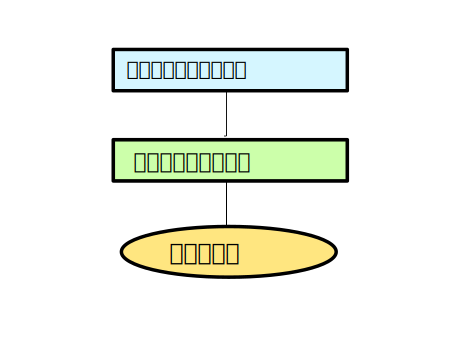
\includegraphics[width=100mm]{experiment_process.png}
\end{center}
\end{frame}

\begin{frame}\frametitle{評価方法}
\begin{block}{ARI (Adjusted Rand Index)}
\begin{itemize}
 \item -1から1までの範囲で精度評価を行う指標
 \item 1の時に完全一致で0の時にランダム
 \item ARIの値が高いほど高評価
\end{itemize}
\end{block}
\begin{center}
\end{center}
\end{frame}

\begin{frame}\frametitle{使用する実データ}
  \begin{block}{Yeast Data Set}
    \begin{itemize}
    \item Yeast(酵母)の形など9属性を収録したデータ
    \item ソース : UCI  Machine Learning Repository
    \item 個体数 : 1484
    \item クラス数 : 10
    \end{itemize}
  \end{block}
\end{frame}

\begin{frame}\frametitle{実験結果}
\end{frame}

\begin{frame}\frametitle{考察}
\begin{itemize}
\item 
\end{itemize}
\end{frame}

\begin{frame}\frametitle{まとめ}
  \begin{block}{目的}
    \begin{itemize}
    \item クラスタリング手法の1つであるFussy c-meansを応用した最適化問題の中から最も精度が高いものを発見する
    \end{itemize}
  \end{block}
  \begin{block}{目標}
    \begin{itemize}
    \item 各クラスタリング手法のプログラムC++を用いて開発
    \item プログラムの実行結果からクラスタリング精度を評価
    \end{itemize}
  \end{block}
  \begin{block}{実験結果}
    \begin{itemize}
    \item 
    \end{itemize}
  \end{block}
  \begin{block}{考察}
      \begin{itemize}
    \item 
    \end{itemize}
  \end{block}
\end{frame}

\end{document}
